%!TEX root = ../thesis.tex
%*******************************************************************************
%****************************** Third Chapter **********************************
%*******************************************************************************

\chapter{Results}

% **************************** Define Graphics Path **************************
\ifpdf
    \graphicspath{{Chapter3/Figs/Raster/}{Chapter3/Figs/PDF/}{Chapter3/Figs/}}
\else
    \graphicspath{{Chapter3/Figs/Vector/}{Chapter3/Figs/}}
\fi

% Oscillations 
\section{The CLV3 domain is periodically regulated}
When tracking the number of CLV3 nuclei identified by Costanza, the results
observable in \cref{fig:clv3_trajs} shows the number of observed CLV3 nuclei
increasing for plants 2, 4, 13, and 15, corresponding to a visually observable
enlargement of the CLV3 domain in \FIG (timelapse of example plant over 4
timepoints?). Similarly, fluctuations in this number can be seen not to 
correlate with the mean expression as described in
\cref{tab:corr_nNucl_meanExpr}. % and therefore ought to be structural

\begin{figure}[H]
  \centering
  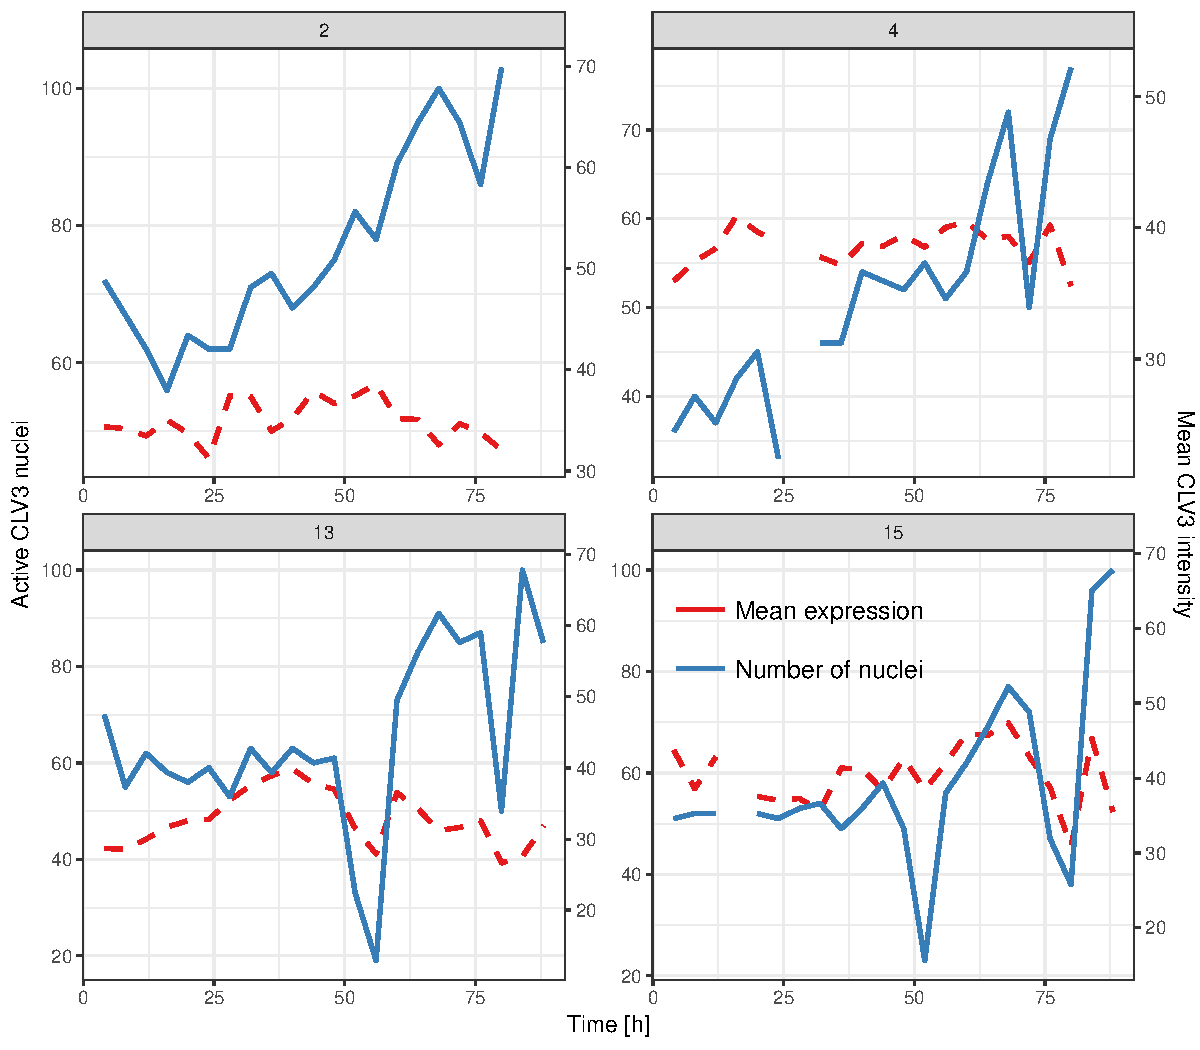
\includegraphics[width=.8\textwidth]{clv3nucl_trajectories.pdf}
  \caption{\todo{Add caption}
  \label{fig:clv3_trajs}
\end{figure}

\begin{table}
  \centering
  \caption{TODO}
  \label{tab:corr_nNucl_meanExpr}
  \begin{tabular}{ll}  \toprule
    Plant & p-value \\ \midrule
    2     & 0.48    \\
    4     & 0.84    \\
    13    & 0.91    \\
    15    & 0.11    \\ \midrule
    All   & 0.50    \\ \bottomrule
  \end{tabular}
\end{table}

In order to assess the extent of the fluctuations the lines were detrended using
a second order Loess fit to each curve. When performing a continuous time
Fourier transform in order to extract amplified modes, the plants have are
biased towards the fourth mode in each respective transformation, as depicted in
\cref{fig:modes}, which corresponds to periodicity of $\sim$16~hours. \FIG
\todo{map this to light / dark hour cycles?}
% and are hence not circadian

In addition to this periodicity, the number of nuclei identified correlated
positively with the number of division events observed in each timepoint for
three out of the four plants. Due to the typical prevalence of loss in nuclear
signal during cellular division



% Trajectories
% Fourier analysis

\section{Epidermal regulation maintains low variance in CZ}

\subsection{Layer-wise separation in the distribution of nuclear volume 
  suggests Epidermal activation}

\subsection{Radial decay in CLV3 expression shows robustness in apical expression}

\subsection{A simple model supports L1 activation hypothesis (hopefully)}

\section{Trajectorial analysis suggests CLV3 decay outside of apex}
This goes in line with previous point. What do I want to say about this? 

\section{Longevity thingy (?)}

\section{Extended data analysis. Include this at all?} 
